\section{Графические иллюстрации}

\begin{frame}[fragile]{Растровые изображения}
	Чтобы вывести растровое изображение из файла необходимо подключить пакет \mintinline{LaTeX}{graphicx} (\mintinline{TeX}{\usepackage{graphicx}}) и команду \mintinline{LaTeX}{\includegraphics}, которая своим обязательным аргументом принимает путь к файлу с изображением. Загруженное изображение воспринимается \LaTeX{} как один большой символ. Необязательный аргумент отвечает позволяет, например, задать размер изображения.
	
\begin{minted}[frame=single, fontsize=\small]{TeX}
Логотип \textbf{python} 
\includegraphics[width=1em]{pictures/python.png} 
изображает в стиле Майа  двух гнездящихся змей.
\end{minted}
	
	Логотип \textbf{python} 
\includegraphics[width=1em]{pictures/python.png}  изображает в стиле Майа  двух гнездящихся змей.
\end{frame}




\begin{frame}[fragile]{Растровые изображения}
	Необязательный аргумент позволяет задавать размер изображения. \mintinline{TeX}{scale} масштабируют относительно исходного изображения. \mintinline{TeX}{width} и \mintinline{TeX}{height} подгоняет размер изображение под заданную ширину или высоту.
	
	\small
	\begin{minted}[frame=single]{TeX}

\includegraphics[scale=0.5]{pictures/python.png}

\includegraphics[scale=2.0]{pictures/python.png}

\includegraphics[width=1em]{pictures/python.png}

\includegraphics[width=2cm, height=1cm]{pictures/python.png}

\includegraphics[width=2cm, height=1cm,
keepaspectratio]{pictures/python.png}
	\end{minted}
	
	
\includegraphics[scale=0.66]{pictures/python.png}
	
\includegraphics[scale=1.5]{pictures/python.png}
	
\includegraphics[width=1em]{pictures/python.png}
	
\includegraphics[width=2cm, height=1cm]{pictures/python.png}
	
\includegraphics[width=2cm, height=1cm, keepaspectratio]{pictures/python.png}
	
\end{frame}

\begin{frame}[fragile]{Растровые изображения}
	\small
	Для того, чтобы растянуть изображение по ширине страницы удобно использовать комбинацию \mintinline{TeX}{width=\textwidth}. 

	\begin{minted}[frame=single, fontsize=\small]{TeX}
\includegraphics[width=\textwidth]{pictures/galaxy.jpg}
	\end{minted}

	\includegraphics[width=\textwidth]{pictures/galaxy.jpg}

	
\end{frame}

\begin{frame}[fragile]{Плавающие иллюстрации}
	\small
\begin{minted}[tabsize=4, frame=single, fontsize=\small]{TeX}
\begin{figure}
	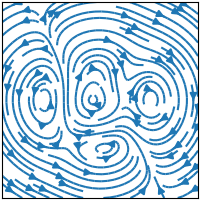
\includegraphics[scale=0.3]{pictures/streamplot.png}
	\caption{Линии тока}\label{fig:streamplot}
\end{figure}
На рис.~\ref{fig:streamplot} построены линии тока функции $f(x, y)$.
\end{minted}
	
	\begin{figure}
		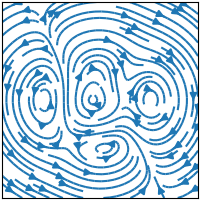
\includegraphics[scale=0.3]{pictures/streamplot.png}
		\caption{Линии тока}\label{fig:streamplot}
	\end{figure}
	На рис.~\ref{fig:streamplot} построены линии тока функции $f(x, y)$.
\end{frame}

\begin{frame}[fragile]{Векторная графика: tikzpicture}
	\small
	
\begin{minipage}{0.69\textwidth}
\begin{minted}[tabsize=4, frame=single, fontsize=\small]{TeX}
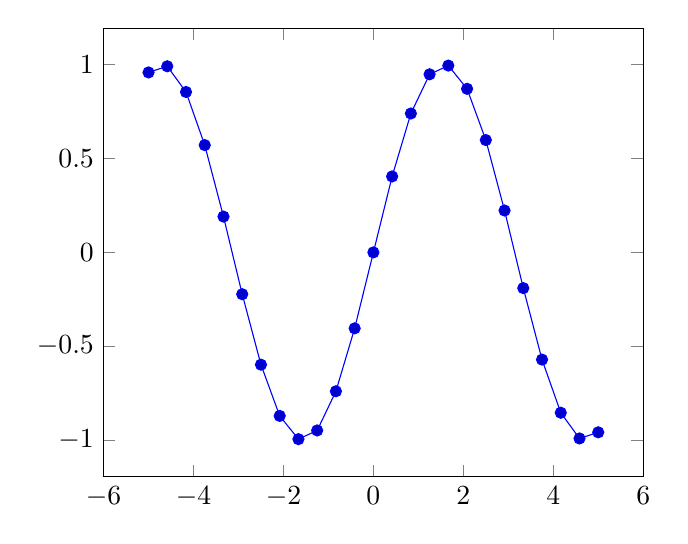
\begin{tikzpicture}
	\begin{axis}
		\addplot {sin(deg(x))};
	\end{axis}
\end{tikzpicture}
\end{minted}
\end{minipage}
	\begin{minipage}{0.29\textwidth}
		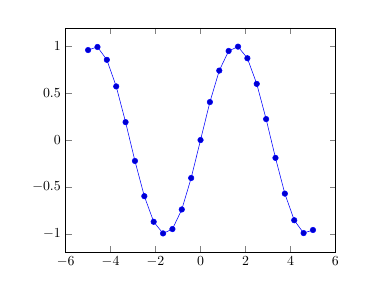
\begin{tikzpicture}[scale=0.5]
			\begin{axis}
				\addplot {sin(deg(x))};
			\end{axis}
		\end{tikzpicture}
	\end{minipage}
	

	
\begin{minipage}{0.69\textwidth}
\begin{minted}[tabsize=4, frame=single, fontsize=\small]{TeX}
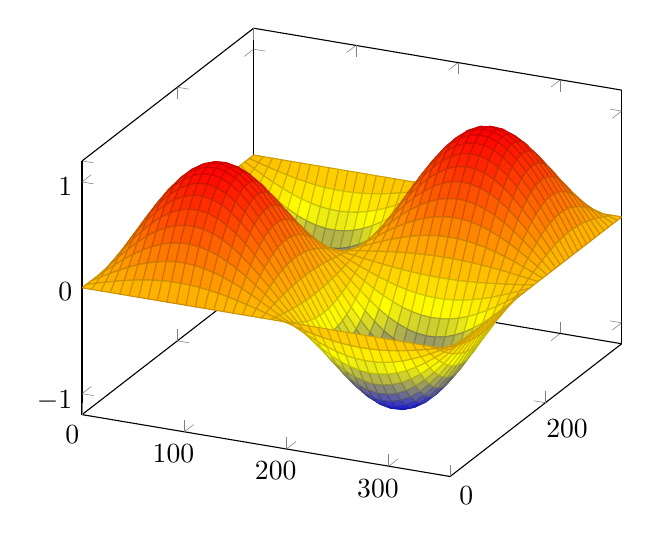
\begin{tikzpicture}
	\begin{axis}
		\addplot3[surf,domain=0:360,samples=40]
		{sin(x)*sin(y)};
	\end{axis}
\end{tikzpicture}
\end{minted}
\end{minipage}
\begin{minipage}{0.29\textwidth}
	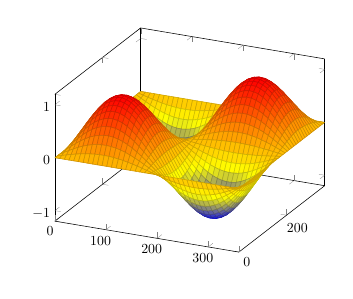
\begin{tikzpicture}[scale=0.5]
		\begin{axis}
			\addplot3[surf,domain=0:360,samples=40]
			{sin(x)*sin(y)};
		\end{axis}
	\end{tikzpicture}
\end{minipage}
	
\end{frame}